\documentclass{article}


% if you need to pass options to natbib, use, e.g.:
%     \PassOptionsToPackage{numbers, compress}{natbib}
% before loading neurips_2023


% ready for submission
\usepackage[final]{neurips_2023}
% \usepackage[nonatbib]{neurips_2023}


% to compile a preprint version, e.g., for submission to arXiv, add add the
% [preprint] option:
%     \usepackage[preprint]{neurips_2023}


% to compile a camera-ready version, add the [final] option, e.g.:
%     \usepackage[final]{neurips_2023}


% to avoid loading the natbib package, add option nonatbib:
%    \usepackage[nonatbib]{neurips_2023}


\usepackage[utf8]{inputenc} % allow utf-8 input
\usepackage[T1]{fontenc}    % use 8-bit T1 fonts
\usepackage{hyperref}       % hyperlinks
\usepackage{url}            % simple URL typesetting
\usepackage{booktabs}       % professional-quality tables
\usepackage{amsfonts}       % blackboard math symbols
\usepackage{nicefrac}       % compact symbols for 1/2, etc.
\usepackage{microtype}      % microtypography
\usepackage{xcolor}         % colors

\usepackage{listings}       % code
\usepackage{graphicx} %插入图片的宏包
\usepackage{float} %设置图片浮动位置的宏包
\usepackage{subfigure} %插入多图时用子图显示的宏包
\usepackage{amsmath}



\title{Bridging the Gap Between Numerical and Categorical Objectives in Time-Series Foundation Models}


\author{
  Yewei Huang \\
  \texttt{istina@sjtu.edu.cn}
}


\begin{document}


\maketitle


\begin{abstract}
Transformer-based time-series foundation models inherit the expressive sequence
modeling structure of large language models, but their loss functions must still
handle the ordered and continuous nature of forecasting targets: some models
predict numerical values directly, while others discretize values and formulate
forecasting as classification, and both choices have distinct advantages and
limitations.  We study this problem through two lightweight adaptations:
changing the fine-tuning objective and replacing the prediction head to switch
between continuous and discretized output formulations.  Experiments on
pretrained Chronos and TimesFM models show that classification-style and
distance-aware objectives can each help, but their effect depends strongly on the
base architecture and evaluation metric.
\end{abstract}


\section{Introduction}

Time series forecasting is a core tool for planning under uncertainty.  It is
used when decisions must be made before future demand, traffic, weather, prices,
or resource consumption are observed.  Classical forecasting methods were built
around explicit statistical structure, including autoregressive integrated
moving-average models and exponential smoothing
\citep{box1970time,winters1960forecasting}.  They remain useful as transparent
baselines.  However, modern applications often require a single model to adapt
across many related series, frequencies, and domains, which has pushed
forecasting toward global neural models and pretrained representations.

Transformers accelerated this shift \citep{vaswani2017attention}.  Earlier
Transformer-based forecasting models adapted attention to long temporal contexts
through efficiency, decomposition, or patching mechanisms
\citep{zhou2021informer,wu2021autoformer,nie2023patchtst}.  More recently,
forecasting foundation models pretrain on broad time-series corpora and transfer
to new datasets with little task-specific data.  TimesFM follows this direction
with a decoder-only architecture for continuous forecasting
\citep{das2024timesfm}.  Chronos takes a more language-model-like route:
continuous observations are scaled, quantized into a finite vocabulary, and then
modeled with Transformer language-model architectures under cross-entropy
\citep{ansari2024chronos}.

These two representative models reveal a basic design tension in time-series
foundation models.  Forecast values are continuous and ordered, so losses such
as mean-squared error, Huber loss, quantile loss, and continuous ranked
probability score naturally reflect numerical distance or distributional
calibration \citep{huber1964robust,koenker1978regression,matheson1976scoring}.
However, purely numerical objectives can also encourage conservative forecasts:
when future trajectories are uncertain or multi-modal, optimizing an average
error may push the model toward a safe central value that is numerically
plausible but not very informative.  At the same time, discretization turns
forecasting into classification, making it compatible with the stable
probabilistic training objectives used by language models.  This can represent
uncertainty more naturally over bins, but plain cross-entropy treats all wrong
classes equally: a token one bin away and a token thousands of bins away receive
the same categorical penalty structure.  Recent work therefore tries to inject
ordinal or distance-aware information into classification-style forecasting
objectives, including Wasserstein-based fine-tuning
\citep{villani2008optimal,chernov2024wasserstein} and ordinal cross-entropy
\citep{wang2025ordinalce}.

This project studies the same objective-design problem from two practical
angles.  First, we keep the pretrained architecture fixed and change the
fine-tuning loss.  For Chronos, whose prediction space is already discretized,
this allows us to compare bin-index regression, Wasserstein-style distances,
CRPS-like objectives, ordinal cross-entropy, and mixtures of cross-entropy and
distance-aware losses without changing the model architecture.  Second, we
modify the prediction head of a pretrained forecasting model.  For TimesFM,
which originally predicts continuous values, this requires adding or replacing a
head so that the same backbone can be optimized with a classification-style
objective.  This route is more intrusive than changing the loss alone, because
it changes the output interface of the pretrained model and can alter the
fine-tuning dynamics.

Our experiments compare these choices on a held-out Monash forecasting dataset
under zero-shot and parameter-efficient fine-tuning settings.  The results do
not support a single universally best objective.  Different losses show
different strengths during fine-tuning, suggesting that objective design remains
an important adaptation choice for pretrained forecasting models.  In addition,
the head-replacement approach can achieve competitive results after fine-tuning,
which indicates that changing the output formulation is also a promising way to
combine classification-style and distance-aware forecasting.  Overall, the
evidence suggests that these objectives are complementary, but their benefit
depends on how they match the pretrained architecture, output representation,
and evaluation metric.

\section{Related Work}

\subsection{Time Series Forecasting}

Given a historical time series $x_{1:T}=(x_1,\ldots,x_T)$, time series
forecasting aims to predict the next $H$ values
$x_{T+1:T+H}$.  A point forecasting model learns a function
\begin{equation}
    \hat{x}_{T+1:T+H}=f_\theta(x_{1:T}),
\end{equation}
while a probabilistic forecasting model estimates a predictive distribution
\begin{equation}
    p_\theta(x_{T+1:T+H}\mid x_{1:T}).
\end{equation}
In practice, this distribution is often represented by samples, quantiles, or a
discretized probability mass over bins.  Classical methods such as ARIMA and
exponential smoothing model this problem with explicit assumptions about
autoregression, trend, and seasonality
\citep{box1970time,winters1960forecasting}.  Recent neural methods instead
learn global representations across many series, and Transformer-based models
have become a common architecture for long-context forecasting
\citep{vaswani2017attention,zhou2021informer,wu2021autoformer,nie2023patchtst}.

\subsection{Chronos}

Chronos is a time-series foundation model that reformulates forecasting as a
language modeling problem \citep{ansari2024chronos}.  Instead of predicting raw
real values directly, it first scales each time series and maps the scaled
values into a fixed vocabulary of discrete bins.  This makes Chronos compatible
with existing Transformer language-model architectures and the standard
cross-entropy objective.  Forecasts are produced by autoregressively sampling
future tokens and mapping them back to numerical bin centers.  This formulation
gives Chronos a clean probabilistic output over possible future values, but it
also inherits a limitation of categorical training: plain cross-entropy rewards
the correct bin without considering the numerical distance between nearby and
far-away mistakes.  This makes Chronos a useful testbed for distance-aware
fine-tuning losses.

\subsection{TimesFM}

TimesFM takes a different route: it is a decoder-only forecasting foundation
model that predicts future values in a continuous output space
\citep{das2024timesfm}.  The model uses patching to compress long time-series
contexts into a shorter sequence of input units, then decodes future patches.
Instead of producing a categorical distribution over token bins, TimesFM outputs
real-valued forecasts for future time steps in a batch.  Its output head
therefore keeps predictions in the original numerical space instead of passing
through a discrete vocabulary.  This preserves the numerical geometry of
forecasting targets, but continuous objectives can also bias the model toward
safe central predictions when the future is uncertain.  TimesFM is therefore
useful for the opposite experiment from Chronos: rather than adding distance
awareness to a classification model, we study whether a continuous forecasting
backbone can benefit from an added or replaced classification-style head.

\subsection{Forecasting Objectives}

The choice of objective determines what kind of forecast the model is encouraged
to produce.  Mean-squared error and Huber loss are numerical objectives that
penalize pointwise forecast errors, with Huber loss reducing the influence of
large deviations \citep{huber1964robust}.  Quantile losses optimize asymmetric
errors for specific quantile levels \citep{koenker1978regression}, while CRPS
evaluates an entire predictive distribution \citep{matheson1976scoring}.
Classification objectives such as cross-entropy optimize the probability of the
correct bin, but ignore numerical distance unless the ordinal structure is added
explicitly.  Recent Wasserstein and ordinal-cross-entropy losses are examples of
this distance-aware direction
\citep{villani2008optimal,chernov2024wasserstein,wang2025ordinalce}.  In our
experiments, these objective families mainly motivate the loss-level fine-tuning
study, while the head-replacement study focuses on switching between the
original continuous objective and cross-entropy over discretized targets.  We
give the concrete definitions of the losses used in our experiments in
Appendix~\ref{app:loss-definitions}.


\section{Method}

\subsection{Overview}

We study two ways to combine classification-style and distance-aware objectives
on pretrained time-series models \citep{ansari2024chronos,das2024timesfm}.  The
first route keeps the pretrained model architecture fixed and only changes the
fine-tuning objective.  This is applied to Chronos, whose output space is already
discretized.  The second route changes the prediction head of a continuous
forecasting model.  This is applied to TimesFM, where we compare the original
continuous head with a newly introduced classification head.

In both routes, the backbone is pretrained; we only change the fine-tuning loss
or the output head before evaluating on held-out series.

\subsection{Loss-Level Fine-Tuning for Chronos}

Chronos converts a real-valued time series into discrete token bins and predicts
a distribution over the bin vocabulary \citep{ansari2024chronos}.  Let $K$
denote the number of numerical bins, $b_t\in\{0,\ldots,K-1\}$ the target bin
index at a valid prediction position, and $p_{t,k}$ the model probability
assigned to bin $k$.  The original Chronos objective is token cross-entropy,
\begin{equation}
    \mathcal{L}_{\mathrm{CE}}
    = -\frac{1}{|\mathcal{M}|}\sum_{t\in\mathcal{M}}\log p_{t,b_t},
\end{equation}
where $\mathcal{M}$ is the set of non-padding target positions.

To inject numerical distance into this discrete output space, we compute losses
in the bin-index space.  The soft prediction is the expected bin index
\begin{equation}
    \bar{b}_t=\sum_{k=0}^{K-1} k\,p_{t,k}.
\end{equation}
The bin-index MSE loss is then
\begin{equation}
    \mathcal{L}_{\mathrm{bin\text{-}MSE}}
    = \frac{1}{|\mathcal{M}|}\sum_{t\in\mathcal{M}}
      \left(\frac{\bar{b}_t-b_t}{K-1}\right)^2 .
\end{equation}
The normalization by $(K-1)^2$ keeps this loss on a comparable scale to
cross-entropy.  We also test a mixed objective that adds a $\lambda$-weighted
CE term to the normalized bin-index MSE.

Beyond MSE, we evaluate several distance-aware losses on the same bin
distribution.  For Wasserstein-style losses, the target is treated as a point
mass at $b_t$ \citep{villani2008optimal,chernov2024wasserstein}:
\begin{equation}
    \mathcal{L}_{W_p}
    = \frac{1}{|\mathcal{M}|}\sum_{t\in\mathcal{M}}
      \frac{\left(\sum_{k=0}^{K-1}p_{t,k}|k-b_t|^p\right)^{1/p}}{K-1},
    \quad p\in\{1,2\}.
\end{equation}
We also use a Huber variant in bin-index space \citep{huber1964robust}.  For
distributional losses, we compare cumulative distributions.  Let
$F_t(k)=\sum_{j\leq k}p_{t,j}$ be the predicted CDF and $G_t(k)$ the target CDF.
The CRPS-style loss uses squared CDF error \citep{matheson1976scoring}, while
ordinal cross-entropy replaces the squared penalty with binary cross-entropy on
the cumulative probabilities \citep{wang2025ordinalce}.  All these losses are
computed only on valid target positions.

\subsection{Head-Level Adaptation for TimesFM}

TimesFM originally predicts future values through a continuous forecasting head
\citep{das2024timesfm}.  We use this original formulation in two ways: as the
zero-shot baseline and as a continuous fine-tuning baseline with LoRA.  We also
train the original forecasting head from scratch as a control.

To study a classification-style output on TimesFM, we add a new CE head on top
of the pretrained backbone.  The backbone first maps patched and normalized
inputs to output embeddings.  The CE head maps each output embedding to
$K$ logits for each future step in the output patch:
\begin{equation}
    \ell_{h,1:K}=g_\phi(r_h),
\end{equation}
where $r_h$ is the TimesFM output representation for horizon step $h$ and
$g_\phi$ is the classification head.  Targets are discretized with uniform bins
over $[-10,10]$ in the RevIN normalized space.  If $\tilde{x}_{T+h}$ is the
normalized target value and
$q(\cdot)$ maps it to a bin index, the CE-head loss is
\begin{equation}
    \mathcal{L}_{\mathrm{TimesFM\text{-}CE}}
    = -\frac{1}{H}\sum_{h=1}^{H}
      \log \operatorname{softmax}(\ell_h)_{q(\tilde{x}_{T+h})}.
\end{equation}

We instantiate this CE head with $K=64$ and $K=256$ bins.  The 64-bin head is
smaller and cheaper to adapt, while the 256-bin head gives a finer
discretization but introduces more output parameters.  In our implementation,
these choices correspond to about 22.6M and 85.6M CE-head parameters,
respectively.  Because the CE head is newly initialized rather than inherited
from the pretrained TimesFM checkpoint, we first pretrain it with the backbone
frozen, then use it for downstream fine-tuning.  We also vary the scale of this
head-pretraining stage: the small pool uses five datasets with 200k sampled
windows, the 256-bin pool uses seven datasets with 200k sampled windows, and the
large-pool 64-bin run uses a larger 300k-window generic pool.

\begin{figure}[H]
    \centering
    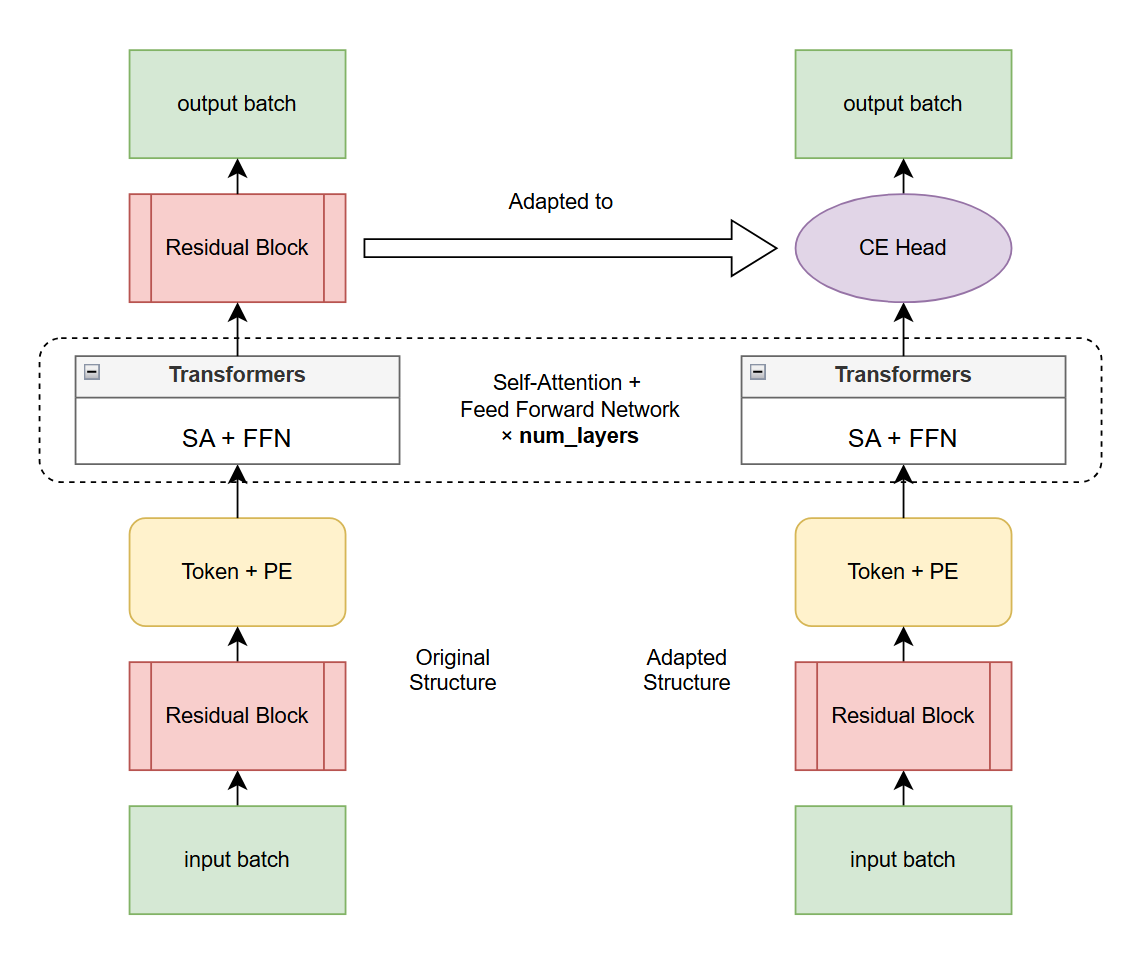
\includegraphics[width=0.76\textwidth]{figures/timesfm-comparison.png}
    \caption{Head-level adaptation for TimesFM.  The original model uses a
    continuous forecasting head, while our adapted version replaces this output
    head with a CE head over discretized targets.}
    \label{fig:timesfm-head-adaptation}
\end{figure}

At inference time, the CE head produces a probability distribution over bins.
We convert this distribution back to numerical forecasts by taking the
softmax-weighted expectation of the bin centers in normalized space and then
applying the inverse RevIN transform.  Quantile forecasts for WQL evaluation are
obtained by inverting the predicted CDF over bins.  Thus the CE head changes the
training target from continuous regression to discretized classification, but
the final outputs are still converted back to real-valued forecasts for
evaluation.

\subsection{Parameter-Efficient Fine-Tuning}

All main downstream experiments use parameter-efficient fine-tuning rather than
full-model training, following the low-rank adapter idea in LoRA
\citep{hu2021lora}.  For Chronos, LoRA adapters are attached to the pretrained
T5 backbone while the loss function is varied.  For TimesFM, LoRA is applied to
the backbone during downstream adaptation, and the output head is trained with a
separate learning rate.  This separation is important for the CE-head setting:
the newly introduced head can adapt much faster than the pretrained backbone,
and using the same aggressive learning rate for both can easily destabilize
fine-tuning.

These two settings cover both directions of the classification-numerical design
choice: adding numerical distance information to a classification model, and
adding a classification head to a numerical forecasting model.

\section{Experiments}

Unless otherwise stated, all reported runs use seed 42.  WQL is computed from
quantile pinball losses, and MASE is a scale-normalized absolute point-forecast
error; lower values are better for both.  Because Chronos and TimesFM use
different split and evaluation pipelines, their absolute scores should be read
within each model family rather than as strict cross-model rankings.

\subsection{Chronos Loss Fine-Tuning}

We first evaluate the loss-level adaptation route on Chronos.  The base model is
\texttt{amazon/chronos-t5-base}.  We use the \texttt{tourism\_monthly} dataset
from the Monash forecasting archive \citep{godahewa2021monash}, with a
sequence-level split of 293 training series and 73 held-out evaluation series.
This dataset is used because it is not part of the listed in-domain Monash
evaluation set for Chronos.  The prediction length is 24, and quantile
evaluation uses 20 generated samples per series.  All fine-tuned Chronos
variants use LoRA adapters; only the fine-tuning objective is changed.  We
report weighted quantile loss (WQL) and MASE.

\begin{table}[H]
    \centering
    \caption{Chronos fine-tuning results on \texttt{tourism\_monthly}.}
    \label{tab:chronos-results}
    \begin{tabular}{lcc}
        \toprule
        Model & WQL & MASE \\
        \midrule
        Zero-shot baseline & 1.5441 & 1.6617 \\
        \midrule
        CE+LoRA & \textbf{1.2244} & 1.3806 \\
        bin-MSE+LoRA & 1.2651 & 1.4176 \\
        bin-MSE+CE+LoRA & 1.2638 & 1.4147 \\
        bin-W1+LoRA & 1.2750 & \textbf{1.3151} \\
        bin-W2+LoRA & 1.3252 & 1.3352 \\
        bin-CRPS+LoRA & 1.2325 & 1.3713 \\
        bin-OrdinalCE+LoRA & 1.2357 & 1.3765 \\
        bin-Huber+LoRA & 1.2562 & 1.3803 \\
        \bottomrule
    \end{tabular}
\end{table}

\begin{figure}[!htbp]
    \centering
    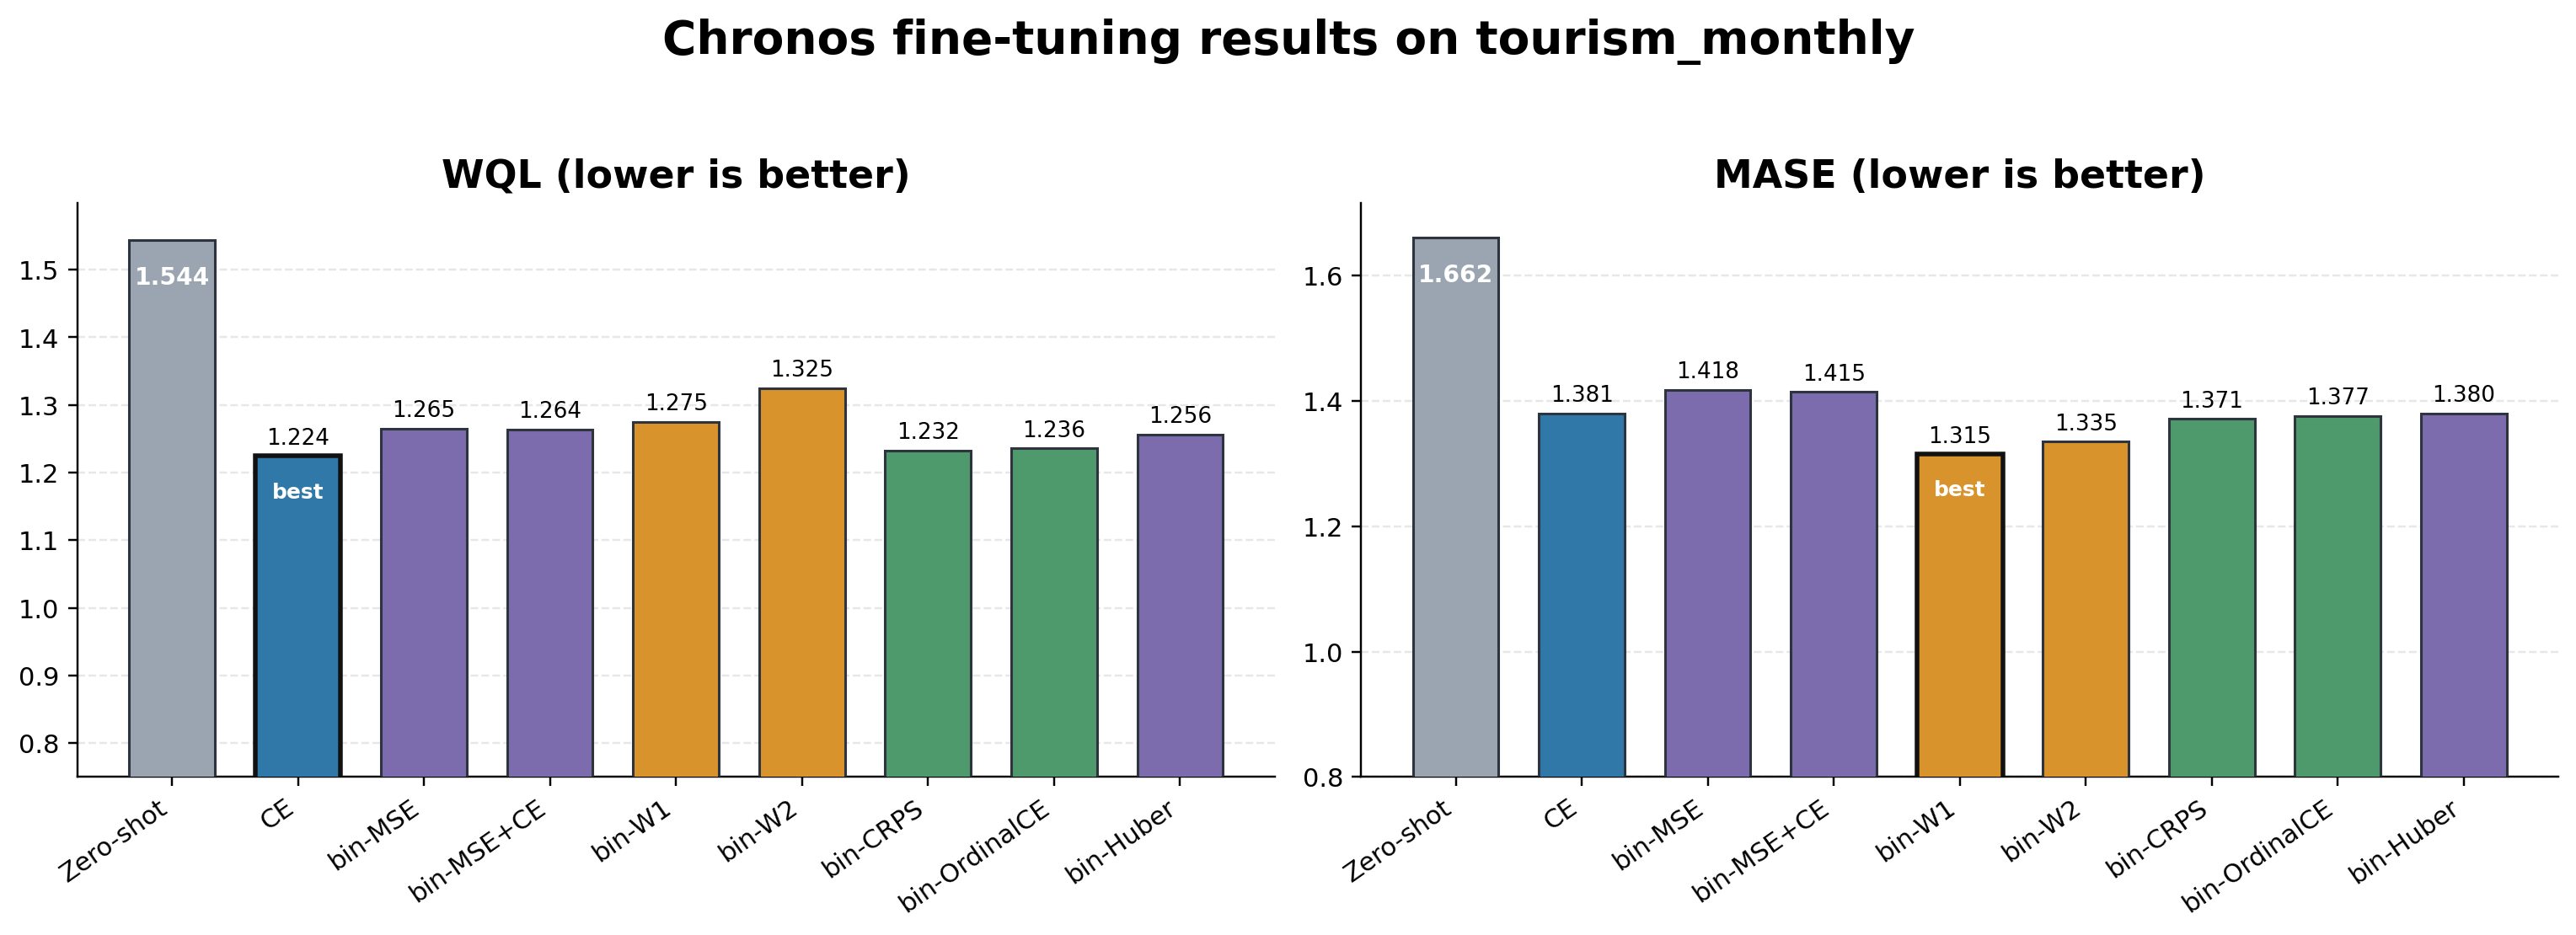
\includegraphics[width=\textwidth]{figures/chronos_metrics_bars.png}
    \caption{Chronos WQL and MASE comparisons.  The zero-shot baseline is
    included as the first bar, while the fine-tuned variants form the main
    comparison.  CE+LoRA obtains the best WQL, while bin-W1+LoRA obtains the
    best MASE.}
    \label{fig:chronos-bars}
\end{figure}

\begin{figure}[!htbp]
    \centering
    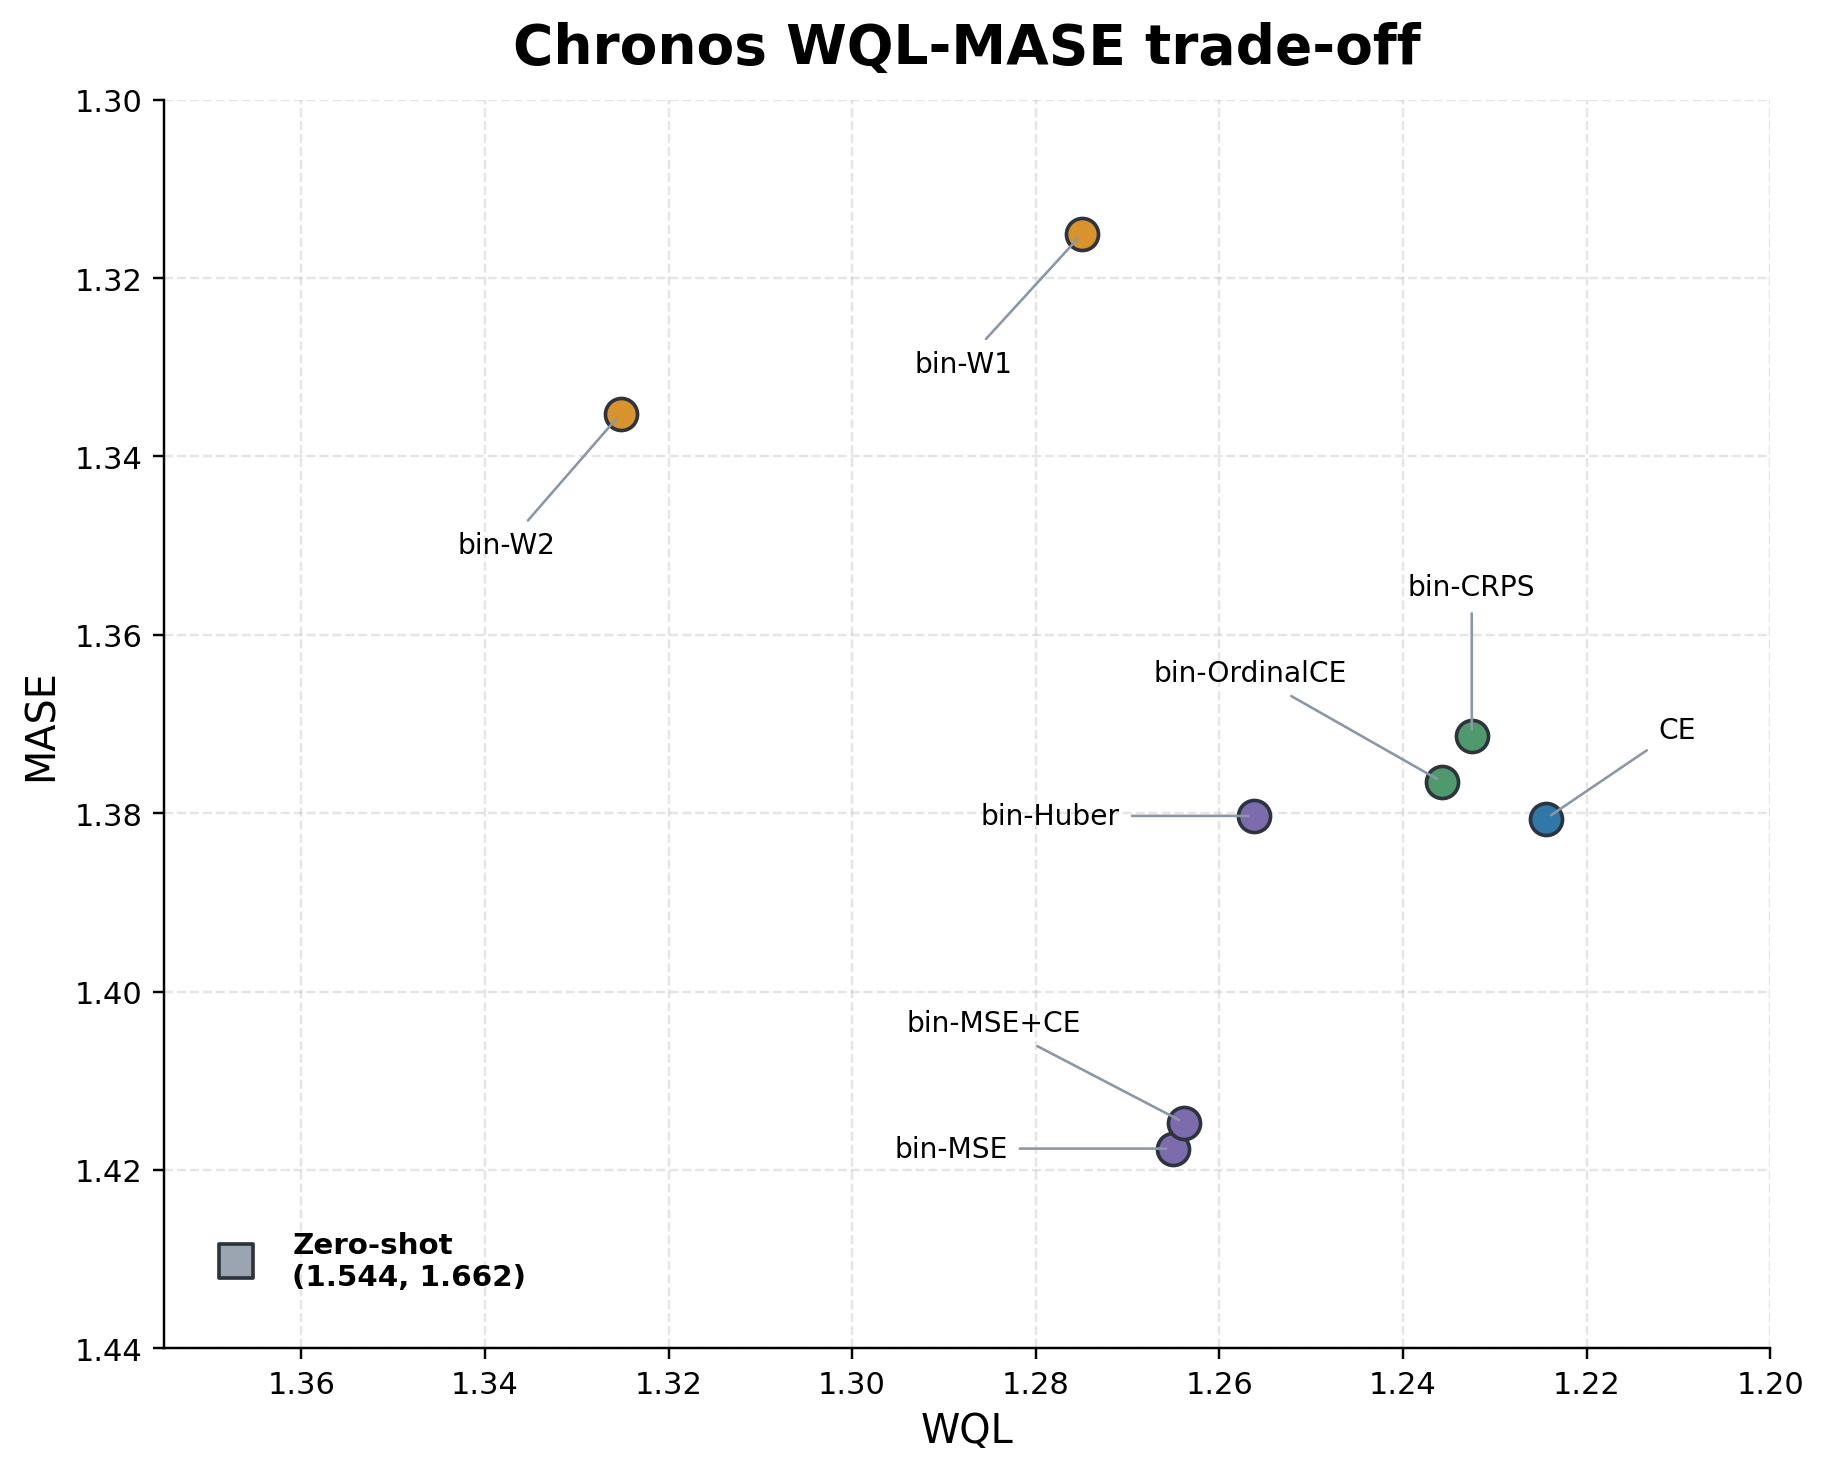
\includegraphics[width=0.78\textwidth]{figures/chronos_wql_mase_scatter.png}
    \caption{Chronos WQL-MASE trade-off.  Different objectives occupy different
    regions of the metric space, showing that the best probabilistic objective
    is not necessarily the best point forecasting objective.  The zero-shot
    baseline is shown as an off-scale reference.}
    \label{fig:chronos-scatter}
\end{figure}

Table~\ref{tab:chronos-results} and Figures~\ref{fig:chronos-bars}
and~\ref{fig:chronos-scatter} summarize the Chronos results.  The zero-shot
baseline records WQL 1.5441 and MASE 1.6617.  All LoRA fine-tuning variants
reduce both metrics.  CE+LoRA obtains the lowest WQL, 1.2244.  bin-W1+LoRA
obtains the lowest MASE, 1.3151.  bin-CRPS+LoRA and bin-OrdinalCE+LoRA are the
next closest variants to CE+LoRA in WQL.  bin-MSE+CE+LoRA remains close to
bin-MSE+LoRA in both metrics.  In the scatter plot, the zero-shot result is
shown as an off-scale reference, and the remaining points compare the
fine-tuned objectives.

\subsection{TimesFM Head Adaptation}

We next evaluate the head-level adaptation route on TimesFM.  The backbone is
\texttt{google/timesfm-2.5-200m-pytorch}.  We do not reproduce the original
Google pretraining of this backbone; instead, our additional pretraining only
trains a replacement output head on selected Monash datasets while keeping the
backbone frozen.  The downstream target is again
\texttt{tourism\_monthly}, but TimesFM uses a different split from Chronos:
257 training series, 36 validation series, and 73 test series.  The context
length is 128 and the prediction length is 24.  To avoid target leakage,
\texttt{tourism\_monthly} is excluded from all head-pretraining pools.

Table~\ref{tab:timesfm-pretrain-data} summarizes the data used for our
replacement-head pretraining.  The small pool was used for the scratch original
forecast head and the 64-bin CE head.  The 256-bin CE head uses the same pool
with two additional monthly datasets.  We also tested a 64-bin CE head pretrained
with a larger generic pool.  All these datasets come from the Monash forecasting
archive \citep{godahewa2021monash}.

\begin{table}[H]
    \centering
    \caption{TimesFM replacement-head pretraining data.  The TimesFM backbone
    itself is loaded from the public pretrained checkpoint; this table only
    describes the additional head-pretraining data used in this project.}
    \label{tab:timesfm-pretrain-data}
    \scriptsize
    \begin{tabular}{p{0.22\textwidth}p{0.52\textwidth}p{0.16\textwidth}}
        \toprule
        Setting & Datasets & Use \\
        \midrule
        small pool &
        \texttt{m4\_monthly}, \texttt{m4\_daily}, \texttt{weather},
        \texttt{electricity\_hourly}, \texttt{traffic\_hourly} &
        original head, CE64 \\
        CE256 pool &
        small pool + \texttt{m3\_monthly}, \texttt{m1\_monthly} &
        CE256 \\
        large pool &
        starter: \texttt{m4\_monthly}, \texttt{temperature\_rain},
        \texttt{weather}, \texttt{traffic\_hourly},
        \texttt{electricity\_hourly}; large: \texttt{kaggle\_web\_traffic},
        \texttt{rideshare}, \texttt{vehicle\_trips}, \texttt{kdd\_cup\_2018},
        \texttt{covid\_deaths}, \texttt{nn5\_daily}, \texttt{fred\_md}, and
        the overlapping M4, weather, traffic, and electricity datasets &
        CE64 large-pool \\
        \bottomrule
    \end{tabular}
\end{table}

For head pretraining, we draw random training windows from the selected
datasets, use a sequence-level validation/test split, and train only the output
head.  The original-head and CE64 runs use 200k random windows, 5 epochs, and a
head learning rate of $10^{-3}$.  The CE256 run also uses 200k windows and 5
epochs, but a smaller batch size because the 256-bin head has many more
parameters.  Downstream LoRA fine-tuning on \texttt{tourism\_monthly} then
updates the backbone adapters and, unless otherwise stated, also updates the
head with a separate learning rate.

\begin{table}[H]
    \centering
    \caption{TimesFM results on \texttt{tourism\_monthly}.  ``Direct'' means
    that the pretrained replacement head is evaluated without downstream
    fine-tuning; ``LoRA'' means downstream fine-tuning on the
    \texttt{tourism\_monthly} training split.  For CE-head rows,
    \texttt{head\_lr} is the output-head learning rate and \texttt{lora\_lr} is
    the backbone-adapter learning rate.  Lower is better.}
    \label{tab:timesfm-results}
    \scriptsize
    \begin{tabular}{p{0.32\textwidth}p{0.38\textwidth}cc}
        \toprule
        Model & Setting & WQL & MASE \\
        \midrule
        Base zero-shot & original TimesFM head & \textbf{1.1899} & 1.1688 \\
        Base LoRA & original regression loss + LoRA, \texttt{lr}=1e-4 &
        1.2058 & 1.1410 \\
        Original head direct & scratch original head, small-pool pretrain &
        1.2795 & 1.2389 \\
        Original head + LoRA & small-pool original head + LoRA, \texttt{lr}=1e-4 &
        1.2049 & 1.1468 \\
        \midrule
        CE64 direct & 64-bin CE head, small-pool pretrain &
        1.4605 & 1.3809 \\
        CE64 + LoRA & \texttt{head\_lr}=5e-5, \texttt{lora\_lr}=5e-5 &
        1.2308 & \textbf{1.1162} \\
        \midrule
        CE256 direct & 256-bin CE head &
        1.3624 & 1.2862 \\
        CE256 + LoRA & \texttt{head\_lr}=1e-5, \texttt{lora\_lr}=5e-5 &
        1.2691 & 1.2336 \\
        \midrule
        CE64 large-pool direct & 64-bin CE head, large-pool pretrain &
        4.5760 & 5.5845 \\
        CE64 large-pool + LoRA & \texttt{head\_lr}=5e-5, \texttt{lora\_lr}=5e-5 &
        1.4641 & 1.3968 \\
        \bottomrule
    \end{tabular}
\end{table}

Table~\ref{tab:timesfm-results} summarizes the TimesFM results.  The base
zero-shot model obtains the lowest WQL, 1.1899.  Base LoRA changes the metrics
to WQL 1.2058 and MASE 1.1410.  The scratch original head obtains WQL 1.2795 and
MASE 1.2389 before downstream LoRA, then WQL 1.2049 and MASE 1.1468 after LoRA.
For the classification heads, CE64 direct records WQL 1.4605 and MASE 1.3809,
while CE64+LoRA records the lowest MASE, 1.1162.  CE256+LoRA with
\texttt{head\_lr}=1e-5 improves over CE256 direct, changing the metrics from
WQL 1.3624 and MASE 1.2862 to WQL 1.2691 and MASE 1.2336.  The CE64 large-pool
head records WQL 4.5760 and MASE 5.5845 before downstream LoRA, then WQL 1.4641
and MASE 1.3968 after downstream LoRA.

\section{Conclusion}

This project studies how loss functions and output formulations affect
pretrained time-series forecasting models.  The Chronos experiments show that
distance-aware fine-tuning is a promising way to improve a categorical
forecasting model, but the distance signal must be expressed in a form that fits
Chronos's discretized output space.  A naive bin-MSE objective by itself is not
the main source of improvement, and mixing it with CE changes little; the
stronger direction is to use losses that operate on the ordered-bin distribution
more directly.  In this setting, bin-W1 achieves the best MASE, while CRPS-style
loss and ordinal CE also improve MASE over CE+LoRA and remain close to CE in
WQL.  These results suggest that Chronos can benefit from numerical geometry
without abandoning its categorical forecasting interface.

The TimesFM experiments point in the opposite direction and lead to the same
broader conclusion.  Starting from a numerical forecasting backbone, adding a CE
head is not a uniformly stronger replacement for the original head: direct CE
transfer is weak, and the base model remains strongest in WQL.  However, CE64
with LoRA substantially improves MASE, showing that the categorical head has
real potential after target-domain adaptation even though it is not the best
overall model in the current setting.  In other words, combining categorical
objectives with numerical forecasting backbones can expose useful behavior that
is not visible under the original output formulation alone.

The results also show a practical trade-off between probabilistic and point
forecasting metrics.  CE keeps a strong advantage for WQL because it directly
optimizes a categorical predictive distribution, while distance-aware losses can
move the model toward better point forecasts by penalizing how far a wrong bin
is from the target.  In Chronos, CE+LoRA obtains the best WQL, whereas bin-W1
obtains the best MASE.  In TimesFM, the original zero-shot model keeps the best
WQL, while CE64 with LoRA obtains the best MASE among our variants.  Rather than
identifying one universal objective, these results show that the useful
objective depends on whether the application values calibrated uncertainty or
accurate point forecasts more.

Overall, the results support the view that forecasting foundation models should
not be tied too rigidly to either pure regression or pure classification
objectives.  A model can benefit from probability mass over discrete outcomes,
from distance-aware numerical structure, or from an architecture that connects
the two.  At the same time, this project is limited by computation and time: we
run the complete pipeline on a single target dataset, so future work should
verify whether the same trends hold across larger and more diverse benchmarks.
The TimesFM results also show that head pretraining data matters.  The
small-pool CE64 head becomes strong after downstream LoRA, but the larger-pool
CE64 head transfers poorly before fine-tuning and remains weak after LoRA.  This
suggests that blindly stacking heterogeneous time-series datasets for head
pretraining can cause severe negative transfer rather than stable improvement.
Since our CE heads are trained only on selected Monash datasets rather than on a
corpus comparable to the original TimesFM pretraining data, stronger and better
matched CE-head pretraining remains an important direction for future work.

\section*{Acknowledgements}

Thanks to AKrry5307 for the inspiration and encouragement throughout this
project.

Thanks to Codex+GPT, Qoder+Qwen, and Kilo Code+DeepSeek for surviving the
debugging, plotting, and paper-polishing loop with me.

\medskip

\bibliographystyle{plainnat}

\bibliography{ref}


\appendix

\section{Loss Definitions}
\label{app:loss-definitions}

This appendix collects the objective definitions referenced in the main text.
Let $\mathcal{M}$ be the set of valid forecast positions, $K$ the number of
bins, $b_t$ the target bin index, and $p_{t,k}$ the predicted probability of bin
$k$ at position $t$.  The standard bin cross-entropy is
\begin{equation}
    \mathcal{L}_{\mathrm{CE}}
    = -\frac{1}{|\mathcal{M}|}\sum_{t\in\mathcal{M}}\log p_{t,b_t}.
\end{equation}
For losses that use a soft numerical prediction in bin space, we use the
expected bin index $\bar{b}_t=\sum_{k=0}^{K-1}k\,p_{t,k}$.  The normalized
bin-index MSE is
\begin{equation}
    \mathcal{L}_{\mathrm{bin\text{-}MSE}}
    = \frac{1}{|\mathcal{M}|}\sum_{t\in\mathcal{M}}
      \left(\frac{\bar{b}_t-b_t}{K-1}\right)^2 .
\end{equation}
The mixed Chronos variant adds a $\lambda$-weighted CE term to this normalized
bin-index MSE.

For Wasserstein-style losses, the target distribution is a point mass at the
target bin:
\begin{equation}
    \mathcal{L}_{W_p}
    = \frac{1}{|\mathcal{M}|}\sum_{t\in\mathcal{M}}
      \frac{\left(\sum_{k=0}^{K-1}p_{t,k}|k-b_t|^p\right)^{1/p}}{K-1},
    \quad p\in\{1,2\}.
\end{equation}
The Huber variant applies the standard Huber penalty to the bin-index error
$e_t=\bar{b}_t-b_t$:
\begin{equation}
    \rho_\delta(e)=
    \begin{cases}
        \frac{1}{2}e^2, & |e|\leq \delta,\\
        \delta\left(|e|-\frac{1}{2}\delta\right), & |e|>\delta.
    \end{cases}
\end{equation}

For CDF-based losses, define the predicted CDF
$F_t(k)=\sum_{j\leq k}p_{t,j}$ and the target CDF
$G_t(k)=\mathbf{1}[k\geq b_t]$.  The CRPS-style loss is
\begin{equation}
    \mathcal{L}_{\mathrm{CRPS}}
    = \frac{1}{|\mathcal{M}|}\sum_{t\in\mathcal{M}}
      \frac{1}{K}\sum_{k=0}^{K-1}\left(F_t(k)-G_t(k)\right)^2 .
\end{equation}
Ordinal cross-entropy uses binary cross-entropy on the same cumulative
probabilities:
\begin{equation}
    \mathcal{L}_{\mathrm{OrdCE}}
    = -\frac{1}{|\mathcal{M}|}\sum_{t\in\mathcal{M}}\frac{1}{K}
      \sum_{k=0}^{K-1}
      \left[
        G_t(k)\log F_t(k)
        + (1-G_t(k))\log(1-F_t(k))
      \right].
\end{equation}

For TimesFM CE-head experiments, the continuous normalized target
$\tilde{x}_{T+h}$ is first mapped to a bin $q(\tilde{x}_{T+h})$, and the head is
trained with the same cross-entropy form over the horizon steps.  Quantile loss,
used in WQL evaluation, is the pinball loss
\begin{equation}
    \rho_\tau(y,\hat{y})
    = \max\{\tau(y-\hat{y}),(\tau-1)(y-\hat{y})\},
\end{equation}
aggregated over the evaluated quantile levels and normalized by the scale of the
target series.


\end{document}
